\section{FPR: 0.01}\label{sec:fpr-001}
\subsection{Setup}\label{subsec:setup}
\begin{figure}[H]
    \centering
    \minipage{0.49\textwidth}
    \includegraphics[width=\linewidth]{openmp/001/setup_times}
        \caption{Speedup setup Omp}\label{fig:setup_time_omp}
    \endminipage\hfill
    \minipage{0.49\textwidth}
    \includegraphics[width=\linewidth]{joblib/001/setup_time_plot}
        \caption{Speedup setup Joblib}\label{fig:setup_time_joblib}
    \endminipage\hfill
\end{figure}
\begin{figure}[H]
    \centering
    \minipage{0.49\textwidth}
    \includegraphics[width=\linewidth]{openmp/001/setup_speedup}
        \caption{Speedup setup Omp}\label{fig:setup_speedup_omp}
    \endminipage\hfill
    \minipage{0.49\textwidth}
    \includegraphics[width=\linewidth]{joblib/001/setup_speedup_plot}
        \caption{Speedup setup Joblib}\label{fig:setup_speedup_joblib}
    \endminipage\hfill
\end{figure}
\begin{figure}[H]
    \centering
    \minipage{0.49\textwidth}
    \includegraphics[width=\linewidth]{openmp/001/setup_fpr}
        \caption{Speedup setup Omp}\label{fig:setup_fpr_omp}
    \endminipage\hfill
    \minipage{0.49\textwidth}
    \includegraphics[width=\linewidth]{joblib/001/setup_fpr_plot}
        \caption{Speedup setup Joblib}\label{fig:setup_fpr_joblib}
    \endminipage\hfill
\end{figure}

In questo contesto, nella fase di setup,
i risultati ottenuti indicano un aumento delle tempistiche di esecuzione per la versione Joblib
rispetto a FP=0.05, tuttavia si osserva un miglioramento in termini di speedup, che raggiunge un massimo di 3.1.
Al contrario, la versione OpenMP manifesta un peggioramento nelle performance di speedup,
raggiungendo un massimo di 7.1 con il massimo numero di thread disponibili.
Anche in questo caso, i valori di FPR (False Positive Rate) sono molto simili tra le due versioni, oscillando intorno
al valore di 0.01.

\subsection{Filter}\label{subsec:filter}
\begin{figure}[H]
    \centering
    \minipage{0.49\textwidth}
    \includegraphics[width=\linewidth]{openmp/001/filter1_times}
        \caption{Times filter Omp}\label{fig:filter_time_omp}
    \endminipage\hfill
    \minipage{0.49\textwidth}
    \includegraphics[width=\linewidth]{joblib/001/filter_time_plot}
        \caption{Times filter Joblib}\label{fig:filter_time_joblib}
    \endminipage\hfill
\end{figure}
\begin{figure}[H]
    \centering
    \minipage{0.49\textwidth}
    \includegraphics[width=\linewidth]{openmp/001/filter1_speedup}
        \caption{Speedup filter Omp}\label{fig:filter_speedup_omp}
    \endminipage\hfill
    \minipage{0.49\textwidth}
    \includegraphics[width=\linewidth]{joblib/001/filter_speedup_plot}
        \caption{Speedup filter Joblib}\label{fig:filter_speedup_joblib}
    \endminipage\hfill
\end{figure}
\begin{figure}[H]
    \centering
    \minipage{0.49\textwidth}
    \includegraphics[width=\linewidth]{openmp/001/filter_fpr}
        \caption{FPR filter Omp}\label{fig:filter_fpr_omp}
    \endminipage\hfill
    \minipage{0.49\textwidth}
    \includegraphics[width=\linewidth]{joblib/001/filter_fpr_plot}
        \caption{FPR filter Joblib}\label{fig:filter_fpr_joblib}
    \endminipage\hfill
\end{figure}

Con l'aumento della precisione del filtro, i risultati ottenuti indicano un leggero peggioramento delle performance,
dovuto al numero maggiore di operazioni da eseguire rispetto a FP=0.05.

\subsection{Chunks}\label{subsec:chunks}
\begin{figure}[H]
    \centering
    \minipage{0.49\textwidth}
    \includegraphics[width=\linewidth]{joblib/001/chunks_time_plot}
        \caption{Times chunks Joblib}\label{fig:chunks_time_joblib}
    \endminipage\hfill
    \minipage{0.49\textwidth}
    \includegraphics[width=\linewidth]{joblib/001/chunks_speedup_plot}
        \caption{Speedup chunks Joblib}\label{fig:chunks_speedup_joblib}
    \endminipage\hfill
\end{figure}

Nella fase di chunking, i risultati ottenuti mostrano un miglioramento delle performance di speedup, raggiungendo un
massimo di 3.3.
Il valore di soglia per il numero di chunk rimane 64, oltre il quale si verifica un declino nelle performance.

\section{FPR: 0.10}\label{sec:fpr-010}
Viceversa vediamo se diminuendo la precisione del filtro, i risultati ottenuti cambiano.

\subsection{Setup}\label{subsec:fpr-010-setup}
\begin{figure}[H]
    \centering
    \minipage{0.49\textwidth}
    \includegraphics[width=\linewidth]{openmp/010/setup_times}
        \caption{Time setup Omp}\label{fig:010-setup_time_omp}
    \endminipage\hfill
    \minipage{0.49\textwidth}
    \includegraphics[width=\linewidth]{joblib/010/setup_time_plot}
        \caption{Time setup Joblib}\label{fig:010setup_time_joblib}
    \endminipage\hfill
\end{figure}
\begin{figure}[H]
    \centering
    \minipage{0.49\textwidth}
    \includegraphics[width=\linewidth]{openmp/010/setup_speedup}
        \caption{Speedup setup Omp}\label{fig:010-setup_speedup_omp}
    \endminipage\hfill
    \minipage{0.49\textwidth}
    \includegraphics[width=\linewidth]{joblib/010/setup_speedup_plot}
        \caption{Speedup setup Joblib}\label{fig:010-setup_speedup_joblib}
    \endminipage\hfill
\end{figure}
\begin{figure}[H]
    \centering
    \minipage{0.49\textwidth}
    \includegraphics[width=\linewidth]{openmp/010/setup_fpr}
        \caption{FPR setup Omp}\label{fig:010-setup_fpr_omp}
    \endminipage\hfill
    \minipage{0.49\textwidth}
    \includegraphics[width=\linewidth]{joblib/010/setup_fpr_plot}
        \caption{FPR setup Joblib}\label{fig:010-setup_fpr_joblib}
    \endminipage\hfill
\end{figure}

In termini di tempo nella fase di setup, i risultati ottenuti indicano un peggioramento delle performance per la
versione OpenMP, rispetto al valore di FPR=0.05.
La versione Joblib, invece, mostra un peggioramento nelle fasi iniziali del test per poi stabilizzarsi intorno al
valore di 2.5 per il massimo numero di thread disponibili.

\subsection{Filter}\label{subsec:fpr-010-filter}
\begin{figure}[H]
    \centering
    \minipage{0.49\textwidth}
    \includegraphics[width=\linewidth]{openmp/010/filter1_times}
        \caption{Time setup Omp}\label{fig:010-filter_time_omp}
    \endminipage\hfill
    \minipage{0.49\textwidth}
    \includegraphics[width=\linewidth]{joblib/010/filter_time_plot}
        \caption{Speedup setup Joblib}\label{fig:010-filter_time_joblib}
    \endminipage\hfill
\end{figure}
\begin{figure}[H]
    \centering
    \minipage{0.49\textwidth}
    \includegraphics[width=\linewidth]{openmp/010/filter1_speedup}
        \caption{Speedup setup Omp}\label{fig:010-filter_speedup_omp}
    \endminipage\hfill
    \minipage{0.49\textwidth}
    \includegraphics[width=\linewidth]{joblib/010/filter_speedup_plot}
        \caption{Speedup setup Joblib}\label{fig:010-filter_speedup_joblib}
    \endminipage\hfill
\end{figure}
\begin{figure}[H]
    \centering
    \minipage{0.49\textwidth}
    \includegraphics[width=\linewidth]{openmp/010/filter_fpr}
        \caption{FPR Filter Omp}\label{fig:010-filter_fpr_omp}
    \endminipage\hfill
    \minipage{0.49\textwidth}
    \includegraphics[width=\linewidth]{joblib/010/filter_fpr_plot}
        \caption{FPR Filter Joblib}\label{fig:010-filter_fpr_joblib}
    \endminipage\hfill
\end{figure}

Per la fase di filtraggio, i risultati risultano essere molto simili a quelli ottenuti con FPR=0.05.

\subsection{Chunks}\label{subsec:010-chunks}
\begin{figure}[H]
    \centering
    \minipage{0.49\textwidth}
    \includegraphics[width=\linewidth]{joblib/010/chunks_time_plot}
        \caption{Times setup Chunk}\label{fig:010-chunks_time}
    \endminipage\hfill
    \minipage{0.49\textwidth}
    \includegraphics[width=\linewidth]{joblib/010/chunks_speedup_plot}
        \caption{Speedup setup Chunk}\label{fig:010-chunks_speedup}
    \endminipage\hfill
\end{figure}

Nella fase di chunking, i risultati ottenuti mostrano come il valore di soglia di chunk sia 256, oltre il quale si
verifica un declino nelle performance.